%!TEX root = ../../tcc.tex

\section{IPv6}

\begin{comment}
O IPv6 é a versão mais recente do protocolo de Internet (IP), que foi criado para
substituir o IPv4, que atualmente é mais o usado porém sofre de exaustão de endereços.
Nesta seção, falarei sobre o novo protocolo e quais as implicações na programação de
softwares com comunicação de redes.
\end{comment}

Com o desenvolvimento da ARPAnet, a quantidade de computadores conectados na rede
cresceu, chegando a 562 em 1983. A quarta versão do protocolo TCP/IP, o IPv4, foi
criado em 1981 \cite{site:rfcipv4}, foi utilizado para organizar aquelas redes já
formadas e ordenar o crescimento posterior.

O IPv4 tem dois objetivos: prover a fragmentação de pacotes maiores em partes menores,
para que pudessem ser enviados pela camada de enlace; e regras de endereçamento, para
que os pacotes tivessem os endereços de origem e de destino armazenados em seus
cabeçalhos \cite{site:nicipv4}. Apesar de ser considerada robusta e de fácil
implantação e interoperabilidade, o projeto original não previu problemas como o
crescimento das redes e das tabelas de roteamento, segurança de dados, prioridade de
entrega de tipos específicos de pacote e, o mais grave, o esgotamento de endereços IP.

O endereçamento do IPv4 é feito com 4 bytes, geralmente representado na forma decimal
(4 números de 0 a 255), separados por pontos, o que permite $2^32$ endereços possíveis.
Esses endereços, que são distribuídos pela IANA
(\emph{Internet Assigned Numbers Authority}) globalmente para os cinco RIRs
(\emph{Regional Internet Registry}, ou Registro Regional de Internet), que então
distribuem localmente para clientes que incluem provedores de Internet (\glspl{isp}) e
outras organizações, que então repassam endereços a usuários finais. Esses endereços
são os que estão esgotando atualmente. Para resolver esse problema e alguns outros
adquiridos com a experiência operacional do IPv4, o IPv6 foi publicado em 1998
\cite{site:rfcipv6}.


\begin{figure}[H]
    \centering
    \fbox{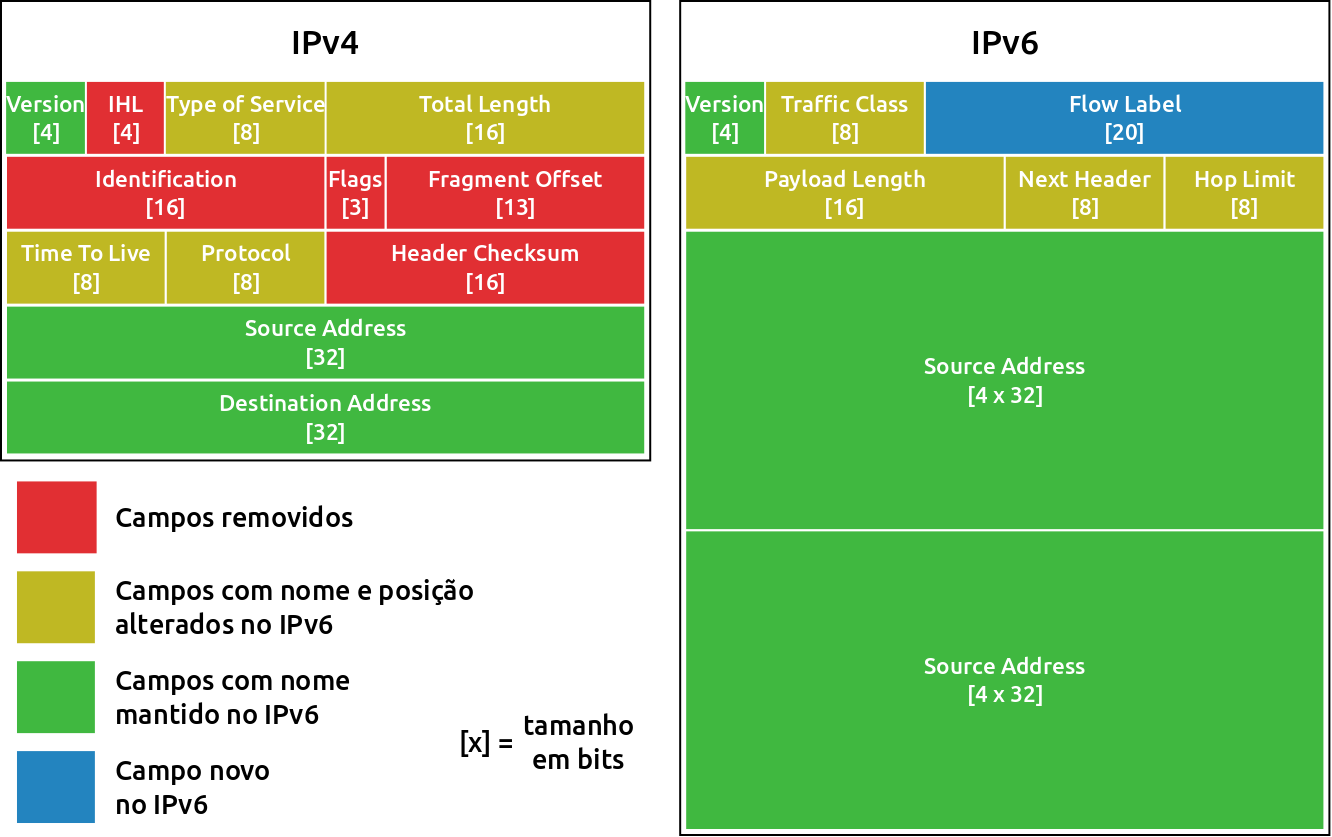
\includegraphics[width=\textwidth]{IPheaders.png}}
    \caption{cabeçalhos de pacotes IPv4 e IPv6, com larguras de 32 bits}
    \label{fig:headers}
\end{figure}